\section{Аналитический обзор литературы}
\label{sec:domain}

В данном разделе будет произведён обзор аналитической литературы, необходимой для рассмотрения непосредственно самой темы, нахождение аналогов и нахождение в них проблемных мест; рассмотрены две архитектуры MVC и Redux; рассмотрен серверный движок Node.js и целесообразность его использования в качестве сервера; приведена оценка нерелятивистких баз данных, их преимущества и недостатки.
Также будут рассмотрены основные фреймворки и инструменты, которые будут использованы в рамках дипломного проекта, и произведено сравнение с существующим ПО для решения схожих задач.

\subsection{Дизайн и пользовательский интерфейс}
\label{sub:domain:bayes_net}
Неотъемлимой частью веб-сайта является его представление и дизайн. За все время развития сети Интернет основы дизайна постоянно менялись, однако это помогло выявить некоторые фундаментальные признаки разработки интерфейсов.

Интерфейс пользователя – это не только его внешний вид. Важной составляющей интерфейса является так называемый “опыт пользователя” – совокупность критериев и факторов, влияющих на взаимодействие пользователя с веб-сайтом. Этими факторами являются краткость и исчерпываемость информации о том, для чего нужен данный сайт; вовлеченность пользователя; однозначность и последовательность действий и др.

Для упрощения разработки таких интерфейсов могут использоваться готовые решения (фреймворки клиентской стороны). Такой подход дает значительное приемущество в скорости разработки, увеличивает переиспользование кода, улучшает его читаемость, а также позволяет получить улучшение производительности засчет внутренних оптимизаций. Также это позволяет сделать веб-сайт единообразным, а следовательно и легко воспринимаемым. Ценой этого является увеличение размера проекта за счет использования сторонних библиотек.

Ключевым моментом веб-сайта является его наполнение. Веб-страница не должна быть перегружена информацией и в то же время пользователь должен без труда найти все то, что ему нужно. Для поиска лучших вариантов наполнения используется подход A/B-тестирования, когда разным группам пользователей отображается разное содержимое страниц. Данные о поведении этих пользователей сохраняются для дальнейшего анализа и принятия решений о содержимом веб-сайта.

%Что такое байесовы сети (2 стр)

\subsection{Реализация дизайна на HTML и CSS}
\label{sub:domain:learning_structure}
При реализации интерфейса и работе с дизайном мы получаем набор черновиков и дизайнов всех веб-страниц разрабатываемого приложения. Следующим этапом является их преобразование в формат, воспринимаемый современными веб-браузерами. Так как пользователей старых веб-браузеров с каждым годом становится все меньше, акцентировать внимание на их поддержке не стоит. Большинство современных браузеров имеют свои собственные алгоритмы отрисовки содержимого, это следует учитывать при разработке каскадных таблиц стилей. Чтобы избежать проблему портирования стилей, следует использовать фреймворки, ориентированные на особенности каждого веб-браузера.

%О важности вывода структуры (1 стр)

\subsection{Серверная архитектура приложения MVC}
\label{sub:domain:manual_structure}
Архитектура программного обеспечения (англ. software architecture) — это высокоуровневая структура программной системы, дисциплина создания таких структур и документация по этим структурам. Архитектура является множеством структур, необходимых для рассуждения о программной системе, и включает элементы системы, связи между ними и свойства этих элементов и связей.

Наиболее популярным подходом при проектировании веб-приложений является архитектура MVC (model-view-controller, модель-представление-контроллер). Основными преимуществами данного подхода являются:

\begin{itemize}
  \item естественность взаимодействия пользователя с системой: пользователь взаимодействует с представлением, а в ответ получает новое представление с обновленными данными модели;
  \item процесс объединения технологий (таких как базы данных, шаблоны страниц и исполняемый код) упрощается за счет разделения их на разные слои (уровень модели, уровень представления и уровень контроллера);
  \item модели, приближенные к реальным, содержат данные, используемые в бизнес-логике, и операции над ними;
  \item представления, используемые для отображения информации пользователю, которые отделены от слоя бизнес-логики;
  \item контроллеры, используемые для обработки запросов пользователя и формирования ответов пользователю используя представления;
\end{itemize}

С учетом всех приведенных выше дополнительных наблюдений, можно построить вид самой архитектуры, которая приведена на рисунке~\ref{fig:domain:manual_structure:credit_net}.

\begin{figure}[ht]
\centering
  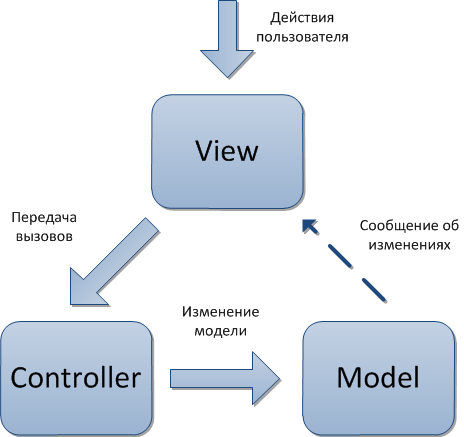
\includegraphics[scale=1]{mvc.png}  
  \caption{ Схема архитектуры MVC. }
  \label{fig:domain:manual_structure:credit_net}
\end{figure}

Таким образом, разбиение на уровни является основным преимуществом использования архитектуры MVC. Её применение будет реализовано на серверной стороне.

% 2 стр

\subsection{Клиентская архитектура приложения Redux}
\label{sub:domain:learning_complexity}

Со стечением времени, архитектура MVC стала слишком громоздкой и её использование во многих веб-приложениях ориентированных, как клиентское приложение становится уже не целесообразно. На её основе начали создаваться улучшенные виды архитектуры и одна из них является Redux.

Redux может быть описан тремя фундаментальными принципами:
 
\begin{itemize}
  \item единственный источник правды. Состояние всего приложения сохраняется в дереве объектов одного хранилища. Это дает возможность создавать универсальные приложения. Состояние на сервере может быть сериализовано и отправлено на клиент без особых трудностей;
  \item состояние только для чтения. Единственный способ изменить состояние – это применить действие – объект, который описывает, что должно случится;
  \item мутации написаны как простые функции. Для определения того, как дерево состояния будет трансформировано действиями, необходимо писать чистые Reducer-функции. Reducer – функции, которые берут предыдущее состояние и действие и возвращает обновленное состояние. Чистая функция – это функция, которая является детерминированной и не обладает побочными эффектами;
\end{itemize}

\begin{figure}[ht]
\centering
  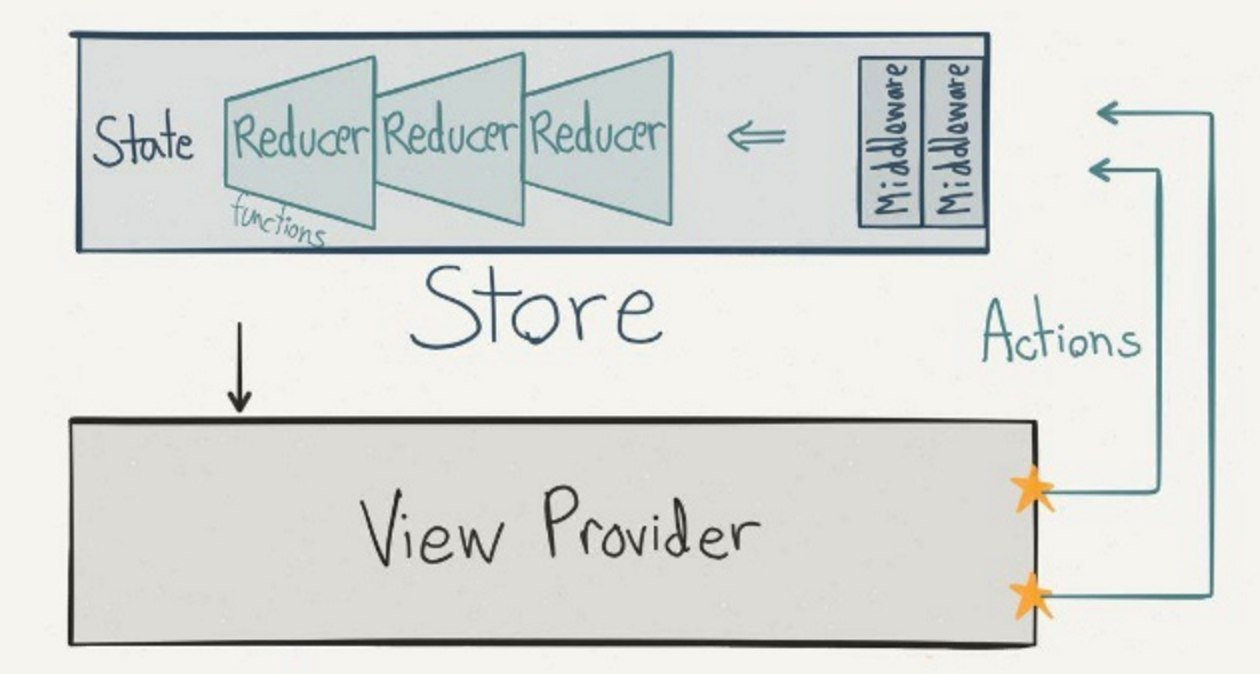
\includegraphics[scale=0.3]{redux.jpg}  
  \caption{ Схема архитектуры Redux. }
  \label{fig:domain:manual_structure:credit_redux}
\end{figure}

На рисунке~\ref{fig:domain:manual_structure:credit_redux}. показана основная схема архитектуры. Разберемся с основными её частями.

Действия (Actions) - это структура, которая передает данные из вашего приложения в хранилище. Они являются единственными источниками информации для хранилища.

Редьюсер (reducer) - это чистая функция, которая принимает предыдущее состояние и действие (state и action) и возвращает следующее состояние (новую версию предыдущего).

Хранилище (Store) - это объект, который соединяет эти части вместе. Хранилище берет на себя следующие задачи:
\begin{itemize}
  \item содержит состояние приложения (application state);
  \item предоставляет доступ к состоянию с помощью getState();
  \item предоставляет возможность обновления состояния с помощью встроенной функции dispatch(action);
  \item регистрирует слушатели (listeners) c помощью subscribe(listener).
\end{itemize}

Таким образом, единственный Store и использование чистых функций является основным преимуществом использования архитектуры Redux.

%Указание что это NP трудная задача (0.5)
%Табличка с оценкой количества сетей в зависимости от числа переменных (для устрашения) (0.2)

\subsection{Платформа Node.js}
\label{sub:domain:mdl_principle}
Node.js является серверной технологией, которая основана на разработанном компанией Google JavaScript-движке V8. Это масштабируемая система, поддерживающая не программные потоки или отдельные процессы, а асинхронный ввод-вывод, управляемый событиями. Она идеально подходит для веб-приложений, которые не выполняют сложных вычислений, но к которым происходят частые обращения.

При использовании обычного веб-сервера, например Apache, при каждом запросе веб-ресурса для обслуживания этого запроса сервер создает отдельный программный поток или вызывает новый процесс. Даже если сервер реагирует на запросы достаточно быстро, а после удовлетворения запроса все приводит в порядок, при таком подходе задействуется множество ресурсов. В результате у наиболее популярных веб-приложений возникают предпосылки для серьезных проблем производительности.

В отличие от этого Node не создает новый программный поток или процесс для каждого запроса, а прослушивает конкретные события, и когда эти события происходят, соответствующим образом на них реагирует. Node не блокирует никаких запросов, дожидаясь завершения действий, инициируемых событием, а сами события обрабатываются в относительно простом цикле обработки событий по принципу «первым пришел — первым обслужен».
Node-приложения создаются с помощью языка JavaScript (или альтернативных языков, компилирующихся в JavaScript), который ничем не отличается от языка, применяемого в приложениях на стороне клиента. Однако в отличие от языка JavaScript, используемого в браузере, для Node нужно создать среду разработки. Node можно установить на платформе Unix/Linux, Mac OS или Windows.

Рассмотрим работу обычного веб-сервера, например Apache. Apache поддерживает две модели мультипроцессорной обработки (Multiprocessing Model, MPM) поступающих запросов. В первой для каждого запроса выделяется отдельный процесс, продолжающийся до тех пор, пока запрос не будет обслужен, во второй для каждого запроса выделяется отдельный программный поток.

В первой MPM-модели, известной как модель prefork, может создаваться столько дочерних процессов, сколько указано в конфигурационном файле Apache. Преимущество создания отдельного процесса состоит в том, что приложения, к которым обращаются посредством запроса, например PHP-приложения, не обязательно должны быть многопоточными. Недостаток заключается в том, что каждый процесс расходует память, и эта модель характеризуется неважной масштабируемостью.

Во второй MPM-модели, известной как модель worker, реализуется гибридная схема процесс-поток, когда каждый поступающий запрос обрабатывается с помощью нового программного потока. С точки зрения расхода памяти этот подход более эффективен, но он требует, чтобы все приложения были многопоточными (то есть были безопасными в отношении потоков). Хотя популярный язык создания веб-приложений PHP теперь безопасен в отношении потоков, нет никаких гарантий, что множество различных библиотек, используемых с интерпретатором этого языка, также безопасно в отношении потоков.

Независимо от используемой модели, запросы обрабатываются в параллельном режиме. Если к веб-приложению в одно и то же время обращается пять человек и сервер имеет соответствующую настройку, все пять запросов обрабатываются одновременно.

В Node все происходит по-другому. При запуске Node-приложения создается единственный программный поток. Node-приложение выполняется в этом потоке в ожидании, что некое приложение сделает запрос. Когда Node-приложение получает запрос, никакие другие запросы не обрабатываются до тех пор, пока не завершится обработка текущего запроса.

Все это кажется не слишком эффективным, если бы не то обстоятельство, что Node работает в асинхронном режиме, используя цикл обработки событий и функции обратного вызова. Цикл обработки событий просто опрашивает конкретные события и в нужное время вызывает обработчики событий. В Node таким обработчиком событий является функция обратного вызова.

В отличие от других однопоточных приложений, когда к Node-приложению делается запрос, оно должно, в свою очередь, запросить какие-то ресурсы (например, обратиться к базе данных или получить доступ к файлу). В этом случае Node инициирует запрос, но не ожидает ответа на этот запрос. Вместо этого запросу назначается некая функция обратного вызова. Когда запрошенное будет готово (или завершено), генерируется событие, активизирующее соответствующую функцию обратного вызова, призванную что-то сделать либо с результатом запрошенного действия, либо с запрошенными ресурсами.

Если пять человек обращаются к Node-приложению в одно и то же время и приложению нужно обратиться к ресурсам из файла, для каждого запроса Node назначает свою функцию обратного вызова событию ответа. Когда для каждого из них ресурс становится доступен, вызывается нужная функция обратного вызова, и запрос удовлетворяется. В промежутке Node-приложение может обрабатывать другие запросы либо для того же приложения, либо для какого-нибудь  другого.

% MDL (2-3)


\subsection{Оценка структуры сети на основе апостериорной вероятности}
\label{sub:domain:k2_algo}
Существуют подходы, использующие байесов метод для оценки качества полученной структуры и алгоритмы на их базе пытаются максимизировать апостериорную вероятность структуры для данного набора экспериментальны данных.
Один из возможных подходов к оценке качества двух структур приведет в работе~\cite{Cooper1991}.
В программном обеспечении, разработанном в данном дипломном проекте, использовался критерий оценки качества структуры, приведенный в упомянутой выше работе.

Введем некоторые обозначения, в дополнение к тем, которые были введены в подразделе~\ref{sub:domain:mdl_principle}.
Пусть структура вероятностной сети обозначается символом $B_S$, таблицы условных распределений, ассоциированные с сетью, "--- $B_P$.
Две вероятностные сети для данного набора экспериментальных данных можно оценить по отношению~(\ref{eq:domain:k2:nets_ratio}) апостериорных вероятностей:
\begin{equation}
  \label{eq:domain:k2:nets_ratio}
  \frac{P(B_{S_i} | x^R[n])}{P(B_{S_j} | x^R[n])} =
    \frac{ \frac{P(B_{S_i}, x^R[n])}{P(x^R[n])} }
         { \frac{P(B_{S_j}, x^R[n])}{P(x^R[n])} } =
    \frac{ P(B_{S_i}, x^R[n]) }
         { P(B_{S_j}, x^R[n]) } \text{\,.}
\end{equation}

Как видно из приведенной формулы~(\ref{eq:domain:k2:nets_ratio}), научившись вычислять отношение совместных распределений, можно сравнивать апостериорные вероятности структур.
Т.\,к. в разработанном ПО использовались результаты, приведенные в работе~\cite{Cooper1991}, то считаем целесообразным привести в данном подразделе базовые формулы и предположения из вышеупомянутой работы.

Для вычисления $P(B_S, D)$ важно сделать несколько важных предположений:

\begin{itemize}
  \item 
  Экспериментальные данные содержат только дискретные случайные величины и все эти случайные величины присутствуют в истинной структуре $B_S$ модели из которой были получены эти экспериментальные данные.
  Из данного предположения следует формула~(\ref{eq:domain:k2:assumption1}):
  \begin{equation}
    \label{eq:domain:k2:assumption1}
    \int_{B_P} P(x^R[n] | B_S, B_P) f(B_P | B_S) P(B_S) dB_p \text{\,,}
  \end{equation}
  \par\hspace{\fivecharsapprox} % абзацный отступ
  \begin{tabular}{@{}ll@{ --- }p{0.74\textwidth}}
  где & $ B_P $ & вектор, содержащий значения условных вероятностей для назначений переменных из структуры $ B_S $; \\
      & $ f $ & условная плотность распределения $B_P$ при условии структуры $B_S$. \\[\parsep]
  \end{tabular}

  \item
  Случаи, зафиксированные в экспериментальных данных, независимы друг от друга, при условии зафиксированной модели, т.\,е. данное предположение подразумевает, что модель, генерирующая экспериментальные данные не меняется.
  Это предположение позволяет упростить формулу~(\ref{eq:domain:k2:assumption1}) и привести её к виду:
  \begin{equation}
    \label{eq:domain:k2:assumption2}
    P(B_S, x^R[n]) =
      P(B_S) \int_{B_P} \left[ \prod_{j = 1}^{n} P(x^R_j | B_S, B_P) \right] f(B_P | B_S) dB_P \text{\,.}
  \end{equation}

  \item
  Экспериментальные данные не должны содержать пропущенных значений для переменных из структуры $B_S$. 
  Введем дополнительные обозначения.
  Пусть $x_j^{(i)}$ представляет значение $i$-й переменной в $j$-м случае.
  Пусть $\phi_i$ представляет из себя вектор уникальных назначений переменных"=родителей для $i$-й переменной, т.\,е. вектор уникальных назначений для $ \forall X_k,\ k \in \pi_i$.
  Пусть $\sigma(i, j)$ индексная функция, которая возвращает индекс назначения $\pi_i$ в $j$-ом случае из вектора $\phi_i$.
  Введем обозначение для длинны вектора $q_i = | \phi_i |$.
  Теперь с учетом предположения об отсутствии пропущенных значений можно вычислить вероятность конкретного случая из экспериментальных данных по формуле:
  \begin{equation}
    \label{eq:domain:k2:case_prob}
    P(x^R_j | B_S, B_P) = 
      \prod_{i = 1}^{R} = P(X_i = x_j^{(i)} | \phi_i[\sigma(i, j)], B_P) \text{\,.}
  \end{equation}
  Подставляя выражение~(\ref{eq:domain:k2:case_prob}) в формулу~(\ref{eq:domain:k2:assumption2}) получим:
  \begin{align}
    \label{eq:domain:k2:assumption3}
    P(B_S, x^R[n]) =
      P(B_S)
      \int_{B_P}\left[ \prod_{j = 1}^{n}\prod_{i = 1}^{R} P(X_i = x_j^{(i)} | \phi_i[\sigma(i, j)], B_P)  \right] &\times \notag\\ 
      \times f(B_P | B_S) dB_P \text{\,.}
  \end{align}
  Пусть для выбранных $i$ и $j$ $f(P(x_i | \phi_i[j], B_P))$ обозначает плотность распределения возможных значений $P(x_i | \phi_i[j], B_P)$.
  Необходимо сделать еще одно предположение.

  \item Для $ 1 \le i, i' \le n$, $ 1 \le j \le q_i $, $1 \le j' \le q_i $, если 
  $ij \neq i'j'$, то распределение $f(P(x_i | \phi_i[j]))$ не зависимо от распределения $f(P(x_{i'} | \phi_{i'}[{j'}]))$.
  Данное предположение по свой сути полагает, что до того, как были получены экспериментальные данные, все возможные назначения равновероятны.
\end{itemize}

С учетом приведенных выше предположений и теоремы, приведённой и доказанной в работе~\cite{Cooper1991}, можно привести формулу для вычисления $P(B_S, D)$:
\begin{equation}
  \label{eq:domain:k2:model_and_data_prob}
  P(B_S, x^R[n]) = 
    P(B_S)
    \prod_{i = 1}^{R}
    \prod_{j = 1}^{q_i}
    \frac{(\alpha_i - 1)!}
         {(n[\phi_i[j], i, B_S] + \alpha_i - 1)!}
    \prod_{k = 1}^{\alpha_i}
      n[v_{ik}, \phi_i[j], i, B_S]! \text{\,,}
\end{equation}
\par
\begin{tabular}{@{}ll@{ --- }p{0.74\textwidth}}
где & $ v_{ik} $ & $k$-е возможное назначение переменной $X_i$. \\[\parsep]
\end{tabular}

Формула~(\ref{eq:domain:k2:model_and_data_prob}) позволяет вычислить значение $P(B_S, x^R[n])$, если известна вероятность $P(B_S)$ и подсчитана оставшаяся часть формулы на основе экспериментальны данных $x^R[n]$.
Но из-за того, что $P(B_S)$ является чаще неизвестной величиной, чем известной, предполагают, что все возможные структуры сети равновероятны и $P(B_S)$ является некой малой константой.
Апостериорную вероятность структуры, при условии данных можно вычислить по формуле:
\begin{equation}
  \label{eq:domain:k2:aposteriori_structure_given_data}
  P(B_S | x^R[n]) = 
    \frac{P(B_S, x^R[n])}
         {\sum_{B_S}P(B_S, x^R[n])} \text{\,.}
\end{equation}

Но, как уже упоминалось, множество возможных структур слишком велико, и на практике значение апостериорной вероятности можно вычислить лишь для малых сетей либо приблизительно. 
В разделе~\ref{sec:arch_and_mod} будет более подробно рассмотрена модификация оценки апостериорной вероятности~(\ref{eq:domain:k2:model_and_data_prob}), применимая на практике.

%Оценка апостериорных вероятностей (K2) (2-3)

\subsection{Общая структура алгоритмов}
\label{sub:domain:other_algos}
В предыдущих двух подразделах были рассмотрены два подхода к оценке качества структуры сети при известных экспериментальных данных.
Как уже упоминалось ранее, выбор функции оценки сети является лишь одним из компонентов большинства алгоритмов построения структуры сети по данным.
Важной частью алгоритма является также выбор стратегии поиска в пространстве возможных структур.
От выбора стратегии поиска зависит трудоемкость алгоритма, качество найденной сети и, собственно, её структура.
В ПО разработанном в рамках дипломного проекта реализовано несколько различных алгоритмов нахождения структуры на основе оценки апостериорной вероятности из подраздела~\ref{sub:domain:k2_algo} и оценки на основе принципа МДО из подраздела~\ref{sub:domain:mdl_principle}.
Стоит упомянуть, что в разработанном ПО реализованы разные стратегии поиска для разных оценок. 
Так алгоритмы использующие оценку МДО могут находить сети произвольной структуры без каких-либо априорных знаний о предметной области.
С другой стороны, для уменьшения пространства возможных решений, алгоритм, использующий оценку апостериорной вероятности, требует априорных знаний об упорядоченности переменных.
В данном конкретном случае, переменные должны быть упорядочены так, что возможные переменные"=родители данной переменной находятся в упорядоченном списке раньше самой переменной.
Во многих других работах накладываются дополнительные ограничения на структуру выводимой сети.
Например, в работе~\cite{Suzuki93} используется оценка МДО, но класс находимых структур ограничен деревьями.
В работе~\cite{Rebane87} приводится алгоритм, ограниченный классом полидеревьев.
% Ограничения других методов построения (упорядоченность нод, ) (2)

\subsection{Обзор существующих программ} % (fold)
\label{sub:domain:existing_programs}
Cуществует множество решений для работы с классическими байесовыми сетями.
Ниже приведены некоторые из задач, которые может выполнять типичный редактор вероятностных сетей:
\begin{itemize}
  \item ручное, автоматическое, полу"=автоматическое построение структуры сети;
  \item оценка параметров условных распределений по данным;
  \item различные алгоритмы статистического вывода суждений в сетях;
  \item генерация экспериментальных данных по готовой сети;
\end{itemize}

Приняв во внимание тему дипломного проекта, наибольший интерес в существуем ПО будет представлять функциональность автоматического вывода структуры сети по данным.
Ниже рассматриваются некоторые из программ для работы с байесовыми сетями.

\subsubsection{SAMIAM }(\url{http://reasoning.cs.ucla.edu/samiam}) 
Бесплатный кросс"=платформенный редактор байесовых сетей, написанный на Java.
Имеет богатую функциональность по ручному созданию сетей.
Поддерживает множество различных алгоритмов вывода статистических суждений и позволяет делать различные типы запросов к сети.
Позволяет генерировать экспериментальные данные, соответствующие готовой сети.
Но функциональность, обеспечивающая автоматический вывод структуры сети по данным, отсутствует.

\subsubsection{Netica }(\url{http://www.norsys.com/netica.html}) 
Коммерческое программное обеспечение.
Версия программы с ограниченной функциональностью свободно доступна на сайте фирмы Norsys.
Netica "--- мощная, удобная в работе программа для работы с графовыми вероятностными моделями. 
Она имеет интуитивный и приятный интерфейс пользователя для просмотра и редактирования топологии сети. 
Соотношения между переменными могут быть заданы, как индивидуальные вероятности, в форме уравнений, или путем автоматического обучения из файлов данных (которые могут содержать пропуски), но, к сожалению, в бесплатном варианте программы данная функциональность недоступна и возможности сравнить с разработанной в дипломном проекте реализацией нет.
Созданные сети могут быть использованы независимо, и как фрагменты более крупных моделей, формируя тем самым библиотеку модулей~\cite{terehov_2003}.

\subsubsection{GeNIe }
\label{sub:domain:existing_programs:genie}
(\url{http://genie.sis.pitt.edu/}) 
Бесплатное кросс"=платформенное приложение и библиотека для работы с вероятностными графовыми моделями, написанная на \cpp{}.
Предоставляется функциональность ручного и автоматического создания сетей, а также реализуются алгоритмы вывода статистических суждений.
Программа реализует несколько алгоритмов вывода структуры сети по данным, целесообразно привести здесь одно небольшое сравнение с разработанным ПО, т.\,к. функциональности приложений пересекаются.
Более подробное сравнение разработанного ПО с существующим будет произведено в разделе~\ref{sec:arch_and_mod}.
Уместно рассмотреть хорошо изученную сеть Asia\footnote{\url{http://www.bnlearn.com/bnrepository/\#asia}}.
Экспериментальные данные, содержащие \num{1000} случаев и имеющие распределение задаваемое сетью, были сгенерированы с помощью одной из вышеперечисленных программ.
К этим экспериментальным данным были применены три различных алгоритма вывода структуры, реализованные в GeNIe.
Выведенные структуры приведены на рисунке~\ref{fig:domain:programs:genie_infered_structrures}.
Для сравнения, структуры, выведенные одним из алгоритмов из разработанной библиотеки на том же наборе данных, и истинная сеть Asia приведены на рисунке~\ref{fig:domain:programs:our_impl_plus_asia}.
Как видно, алгоритм из разработанной библиотеки не нашел одну связь, в отличие от алгоритмов реализованных в GeNIe, которые допустили больше ошибок в структуре.

\begin{figure}[ht]
\centering
  \begin{subfigure}[b]{0.51\textwidth} 
    \centering
    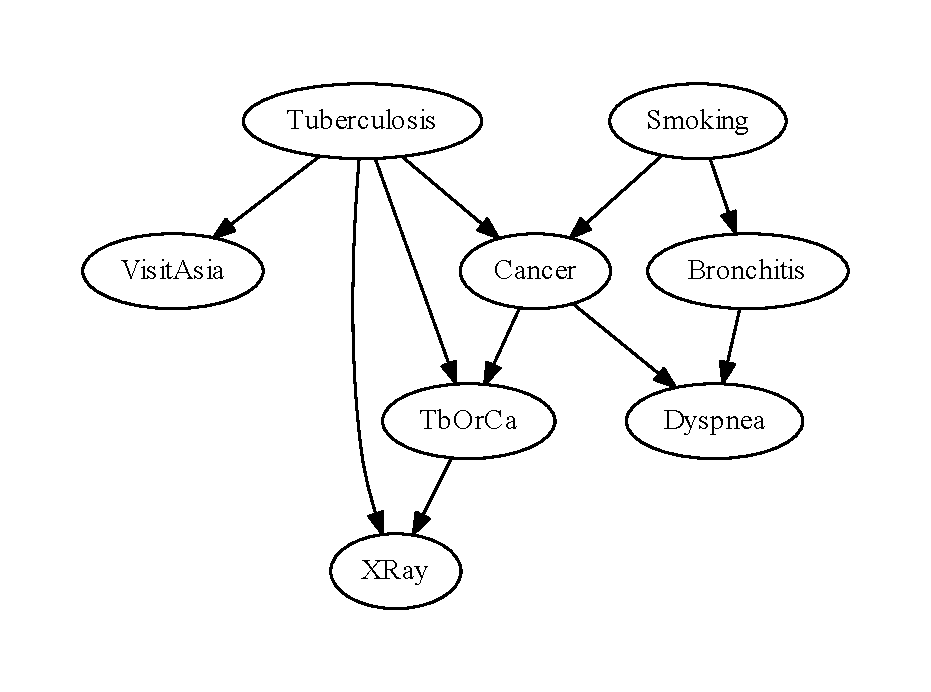
\includegraphics[scale=0.5]{asia_genie_1000_bayesian_search.pdf}  
    \caption{}
  \end{subfigure}
  \begin{subfigure}[b]{0.48\textwidth} 
    \centering
    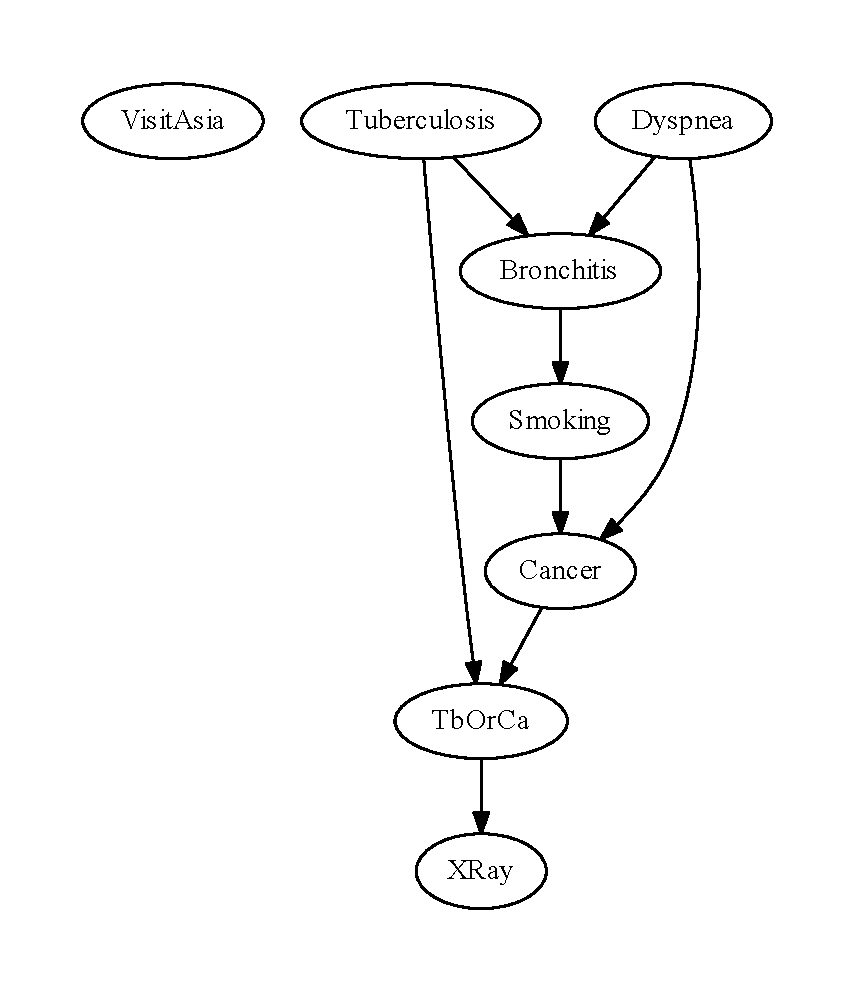
\includegraphics[scale=0.5]{asia_genie_1000_k2.pdf}  
    \caption{}
  \end{subfigure}
  \begin{subfigure}[b]{0.9\textwidth} 
    \centering
    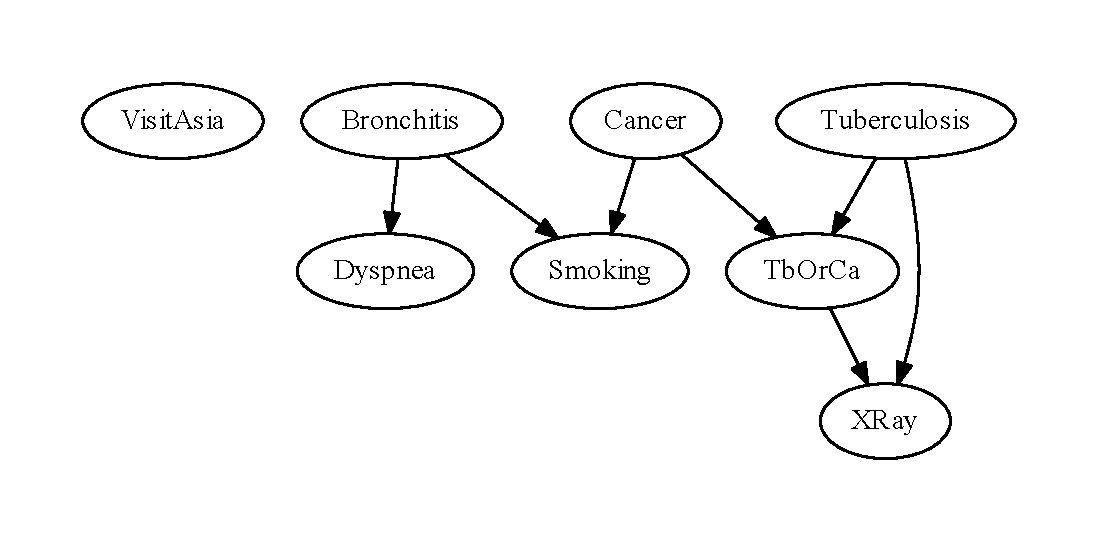
\includegraphics[scale=0.5]{asia_genie_1000_pc.pdf}  
    \caption{}
  \end{subfigure}
  \caption{ Структуры, выведенные по данным с помощью GeNIe: а "--- алгоритм Bayesian Search;
            б "--- алгоритм K2;
            в "--- алгоритм PC;}
  \label{fig:domain:programs:genie_infered_structrures}
\end{figure}


\begin{figure}[ht]
\centering
  \begin{subfigure}[b]{0.49\textwidth} 
    \centering
    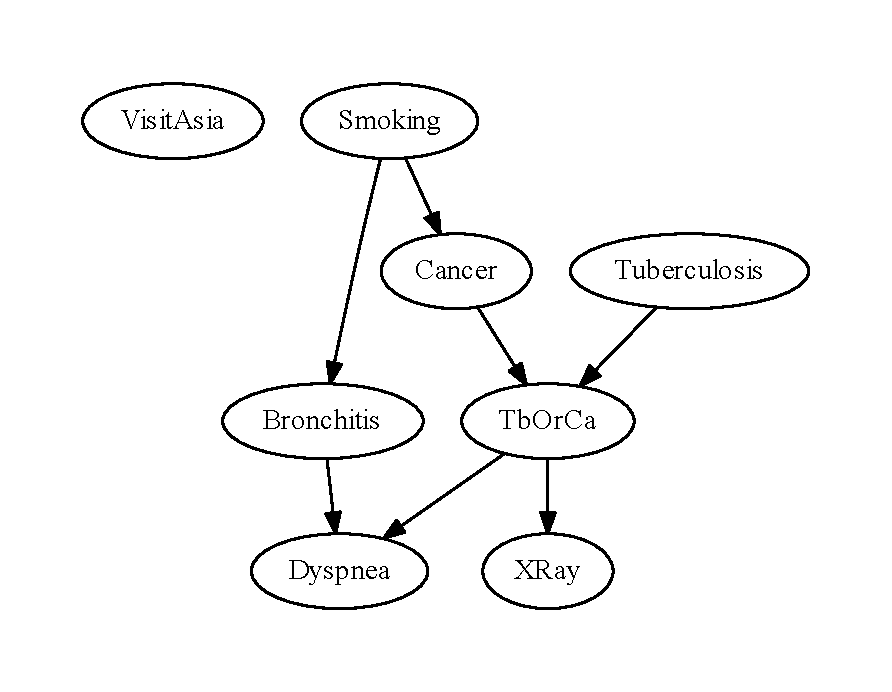
\includegraphics[scale=0.45]{asia-learned-by-terent-random-1000.pdf}  
    \caption{}
  \end{subfigure}
  \begin{subfigure}[b]{0.48\textwidth} 
    \centering
    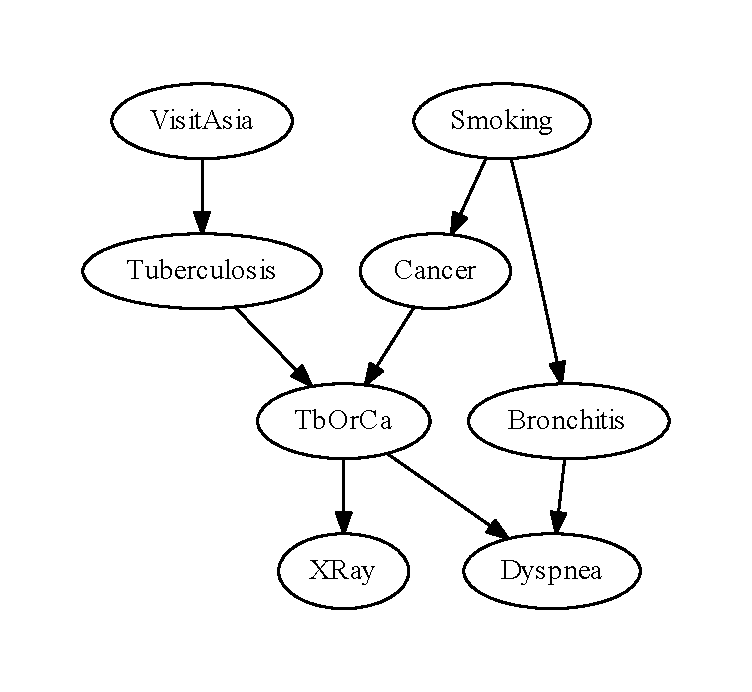
\includegraphics[scale=0.45]{asia_reference_net.pdf}  
    \caption{}
  \end{subfigure}

  \caption{ Выведенная из данных и оригинальная сеть Asia: а "--- алгоритм из разработанной библиотеки, использующий оценку МДО;
            б "--- истинная сеть Asia}
  \label{fig:domain:programs:our_impl_plus_asia}
\end{figure}